\section{Συναρτήσεις κατακερματισμού} \label{section:2-1-hash-functions}

Οι κρυπτογραφικές συναρτήσεις κατακερματισμού (cryptographic hash functions) είναι ειδική κατηγορία συναρτήσεων κατακερματισμού σχεδιασμένες για χρήση στην κρυπτογραφία. Αποτελούν μαθηματικές συναρτήσεις που δέχονται ως είσοδο δεδομένα τυχαίου μεγέθους και επιστρέφουν συμβολοσειρές σταθερού μήκους.

\begin{figure}[H]
	\centering
	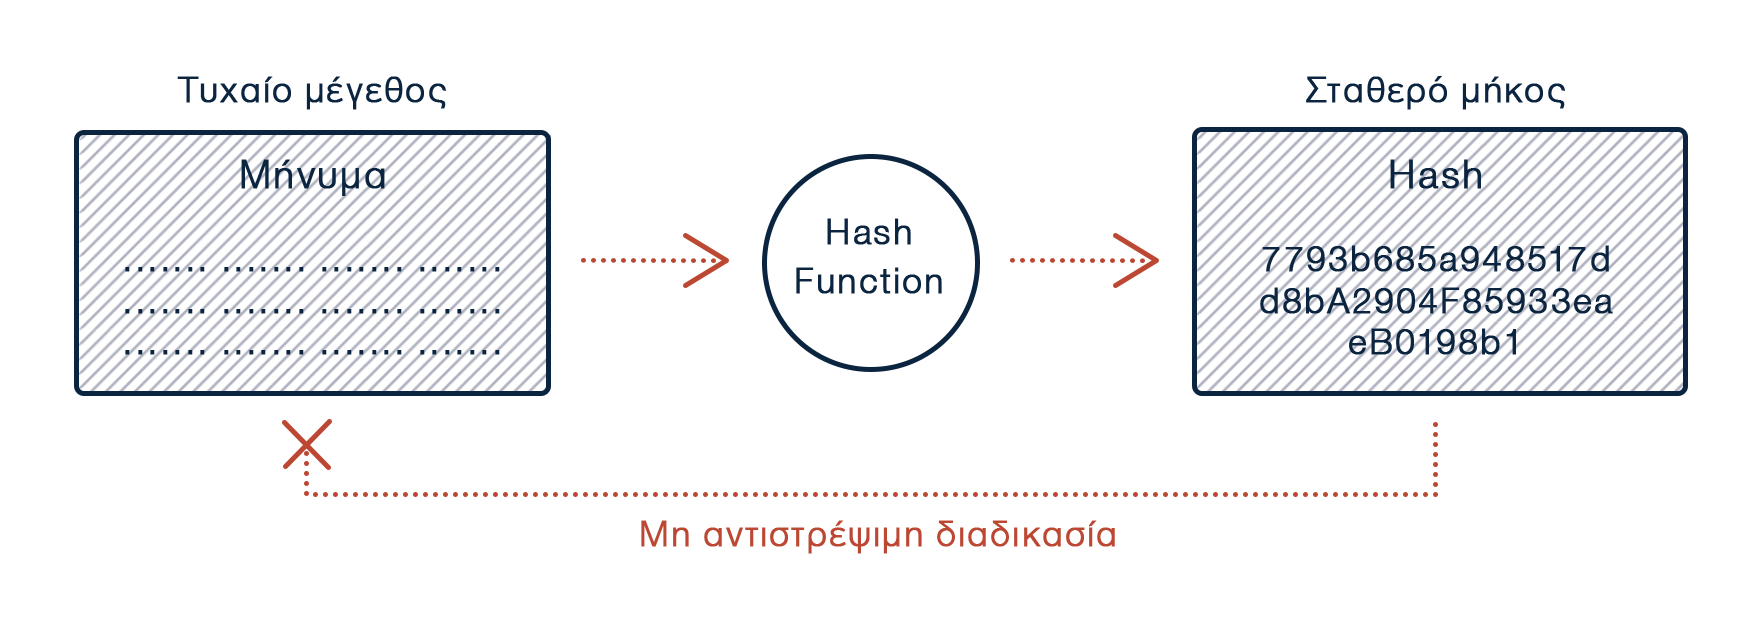
\includegraphics[width=.9\textwidth]{assets/figures/chapter-2/2.1.hash-functions-1.png}
	\caption{Λειτουργία συνάρτησης κατακερματισμού}
\end{figure}

Οι τιμές που επιστρέφει η συνάρτηση κατακερματισμού ονομάζονται τιμές κατακερματισμού (hash values, digests ή απλά hashes). Μία ιδανική κρυπτογραφική συνάρτηση κατακερματισμού έχει τις εξής βασικές ιδιότητες:

\begin{itemize}
	\item Είναι ντετερμινιστική, δηλαδή η ίδια είσοδος παράγει πάντα την ίδια έξοδο.
	\item Είναι μη αντιστρέψιμη, δηλαδή είναι πρακτικά ανέφικτο να υπολογιστεί η είσοδος δεδομένης μιας εξόδου.
	\item Είναι αμφιμονοσήμαντη (1-1), δηλαδή σε δύο διαφορετικές εισόδους αντιστοιχούν πάντα δύο εντελώς διαφορετικές έξοδοι.
	\item Είναι αποδοτική, δηλαδή ο υπολογισμός του hash οποιασδήποτε εισόδου είναι γρήγορος.
\end{itemize}

\begin{figure}[H]
	\centering
	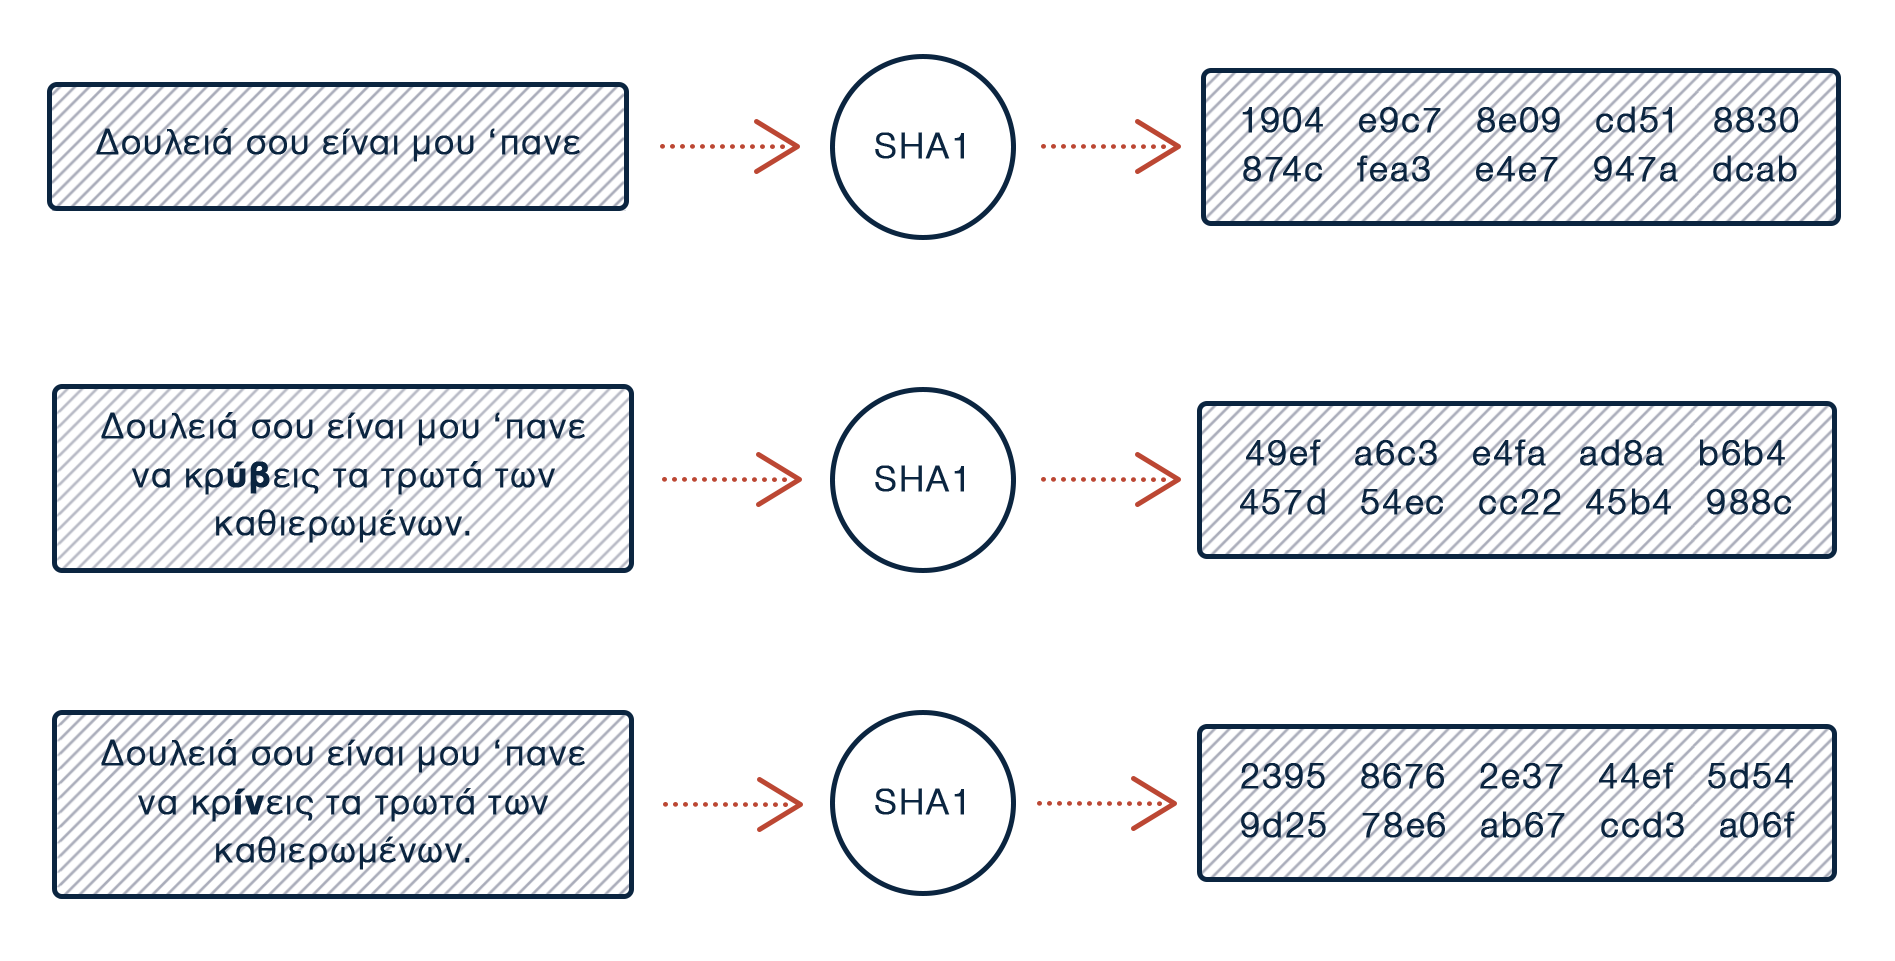
\includegraphics[width=.9\textwidth]{assets/figures/chapter-2/2.1.hash-functions-2.png}
	\caption{Παράδειγμα λειτουργίας συνάρτησης κατακερματισμού}
\end{figure}

Μία από τις δημοφιλέστερες οικογένειες κρυπτογραφικών αλγορίθμων κατακερματισμού είναι αυτή των Secure Hash Algorithms (SHA), η οποία περιλαμβάνει τους SHA-0, SHA-1, SHA-2 και SHA-3.